% This is not in the format for the VUW thesis.
% It is only the rough draft, at this stage.

\documentclass[a4paper]{report}

\usepackage{amssymb, amsmath}
\usepackage{tikz}

\author{Nat Lund}
\title{Chapter 2: Does Slip Exist?}

\newcommand{\beff}{\ensuremath{b_{\mathrm{eff}}}}

\newcommand{\ewf}{\ensuremath{\epsilon_{\mathrm{wf}}}}

\newcommand{\paper}[1]
         {\colorbox[gray]{0.8}{ \textsc{#1}}
         
         }

\begin{document}
\maketitle

If the reader is confident that fluid slip exists, then this chapter may be skipped.  Alternatively, if the slip length is accepted as a being merely a parameter in a mathematical model, and only the mathematical solutions are of interest, then this chapter is superfluous.

However, practical applications of an effective slip length formula require some kind of slip effect to physically exist.  Establishing that a slip effect exists on clean, atomically flat surfaces is far from trivial.  Therefore, in this chapter we will dig quite deeply into the literature on the experimental and theoretical evidence for slip.

%The work of this thesis is predicated on the existence of slip. Therefore, we will examine experimental and %theoretical evidence for slip in the literature.  
This cannot be a comprehensive review of all available literature -- partly because some articles are paywalled -- but rather will be a sample of some high-profile papers.
An exhaustive review of the experimental literature is available in the 2005 review article by Neto \emph{et al} \cite{NetoReview2005}. Other comprehensive reviews are by Vinogradova in 1999 \cite{VinogradovaReview1999} and Lauga, Brenner and Stone in 2006 \cite{LaugaReview2006}. A reasonable introduction is the progress article of Granick \emph{et al} from 2003 \cite{GranickReview2003}.

\section*{Types of Slip}

So far, we have discussed slip within a mathematical model of fluid flow; this is deliberate: in such a model the concepts of slip and slip length are straightforward and intuitive. However, we now need to tackle slip in the real world, disentangling a partially-ordered hierarchy of concepts.

\subsubsection*{Slip Effect}

We begin by considering the concept of a most general slip \emph{effect.} A surface may be described as exhibiting slip if it behaves \emph{as if} fluid slipped on the surface.  For example, for a given pressure, a tube may flow liquid at a rate \emph{as if} it were slightly wider; hence, we could consider it to have a non-zero slip length. But this says nothing about the real conditions on the fluid-solid boundary in the tube. We simply don't know what the fluid velocity at the boundary is. It is possible that the boundary velocity is non-zero, or there may be other effects causing the increased flow. All we can say is that there is a `slip effect'.

\subsubsection*{Intrinsic Slip}

Next, we turn our attention to the \emph{material} of the surface exhibiting  slip effect. Suppose we can prepare a perfectly clean, atomically flat sample of the material. Further, suppose we can experimentally test the sample for slip effects with some pure liquid (pure water, say). If the slip effect still appears, and is replicable, then the implied slip length is a meaningful, reliable parameter of the fluid/solid system. It is reasonable to label this the \emph{intrinsic} slip length.

\subsubsection*{Molecular Slip}

Thus, in the foregoing, slip length is \emph{imputed} to the surface: we \emph{regard} the surface as having a slip length. What would it mean to \emph{really} have a finite slip length? To say anything about the velocity at the surface, we must assume that velocity is well defined. The soothing infinitely-divisible continuum of our model must be replaced with a statistical mechanical definition: the average velocity of some suitable ensemble of \emph{molecules.} Hence, `true' slip entails fluid molecules in some sense sliding over solid molecules. Start by considering a molecule incident on a surface: it has some velocity in the direction tangential to the surface; likewise if it leaves the surface. It is easier to first consider the condition of no slip, then relax that condition. No slip suggests that fluid molecules \emph{stick} to the surface, and if they release, they leave at a \emph{random} angle to the surface, so that the \emph{average} tangential velocity of detaching molecules is the same as the velocity of the surface. Slip suggests, then, that molecules leave the surface with a tangential velocity that \emph{correlates} with the tangential velocity at which they impacted. (Perfect correlation is of course specular reflection --- corresponding to perfect slip, or infinite slip length.) A sensible term for this phenomenom is \emph{molecular slip.}

\subsubsection*{Apparent Slip}

While slip effects are generally acknowledged, the existence of molecular slip remains debatable. Perhaps the simplest alternative to molecular slip to explain slip effects is apparent slip. The idea is that there exists a \emph{boundary layer} of reduced viscosity at the solid surface. As a consequence of the lower viscosity, the velocity gradient in the boundary layer is \emph{steeper} than in the bulk. Thus, the velocity gradient `turns a corner' at the interface between boundary layer and bulk. The no-slip condition holds at the solid/liquid interface, but the velocity gradient in the bulk can be extrapolated to generate a slip length.

The boundary is very thin compared to experimental length scales. The reduction in viscosity is commensurate with a reduction in density; indeed, de Gennes notes that observed slip effects are explainable by a \emph{gas} layer, only 1 or 2 atoms thick. 

\vspace{1em}

\begin{center}
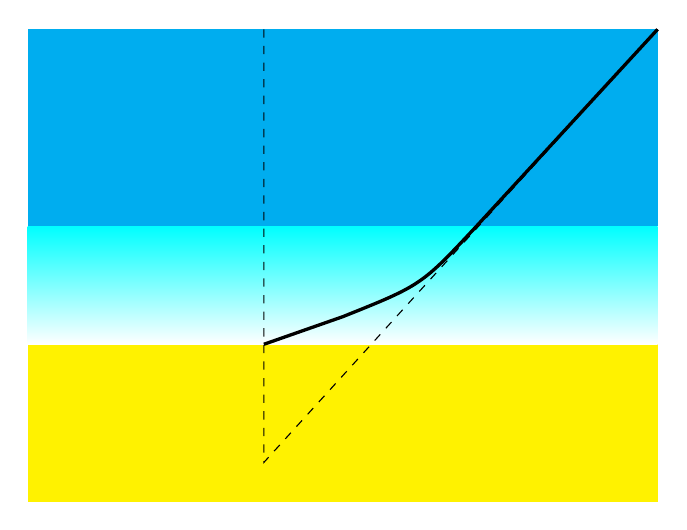
\begin{tikzpicture}

\fill[color=yellow] (-3,-2) rectangle (5,0);

\fill[color=cyan] (-3,1.5) rectangle (5,4);
\shade [top color=cyan] (-3,0) rectangle (5,1.5);

\draw[dashed] (0,4) -- (0,-1.5) -- (5,4);

\draw[very thick] (0,0)--(1.0,0.35) .. controls (2, 0.75) .. (2.7,1.5)--(5,4);

\end{tikzpicture}
\end{center}

\subsubsection*{Effective Slip}

Coming full circle back to a general slip effect, suppose we \emph{know} that the surface under test is not a pure surface.  Then we do not consider the implied slip length to be intrinsic. Instead, we label this the \emph{effective} slip length. This is Nature's average of the intrinsic slip lengths of the system.


\subsubsection*{Measured Slip}

Finally, as we shall see shortly, all measurements are to some extent indirect: Experiments cannot yet directly probe the fluid velocity in the region within a few nanometers of the surface. A measurement of a slip effect may be measuring molecular slip, apparent slip, or, for a heterogeneous surface, any combination of the two.


\subsection*{Definitions in the Literature}

The 2006 review article by Lauga, Brenner and Stone \cite{LaugaReview2006} proposes the following definitions (some paraphrased):

\begin{itemize}

\item \textbf{Phenomenon of slip:} A fluid dynamics system behaving as if the fluid velocity at the wall differs from the wall velocity.

\item \textbf{Molecular slip} (also intrinsic slip): `Refers to the possibility of using hydrodynamics to force liquid molecules to slip against solid molecules.'

\item \textbf{Apparent slip:} The case when the no-slip condition holds on the surface, but at larger length scales, the no-slip condition appears not to be valid.

\item \textbf{Effective slip:} `Refers to the case where molecular or apparent slip is estimated by averaging an appropriate measurement over the length scale of an experimental apparatus.'

\end{itemize}

It may not be immediately clear whether these definitions are compatible with ours, or not. The relationship is clarified once we note that the Lauga \emph{et al} definitions implicitly assume a \emph{homogeneous} surface. Therefore, they define effective slip to be an indirectly measured slip length of a pure surface. The measured slip must then be due to either molecular slip or apparent slip.

By contrast, we explicitly allow a mixed-slip surface. Thus, a measured slip length may be either 1) an effective slip length, or 2) an intrinsic slip length, if we are confident that the surface is pure and uncontaminated. Thus, we redefine effective slip for use on mixed-slip surfaces, and redefine intrinsic slip as pertaining to surfaces that we \emph{know} to be homogeneous.
Hence, the Lauga \emph{et al} use of the phrase `effective slip' falls under our definition of the indirectly measured slip length of a homogeneous surface --- that is, our definition of intrinsic slip. Obviously, we now distinguish between intrinsic and molecular slip. Our definitions of molecular slip are the same.

\clearpage

\subsection*{Types of Slip Redux}

We summarize the hierarchy of slip concepts in the following diagram:

\vspace*{1em}
%.\\
\begin{center}
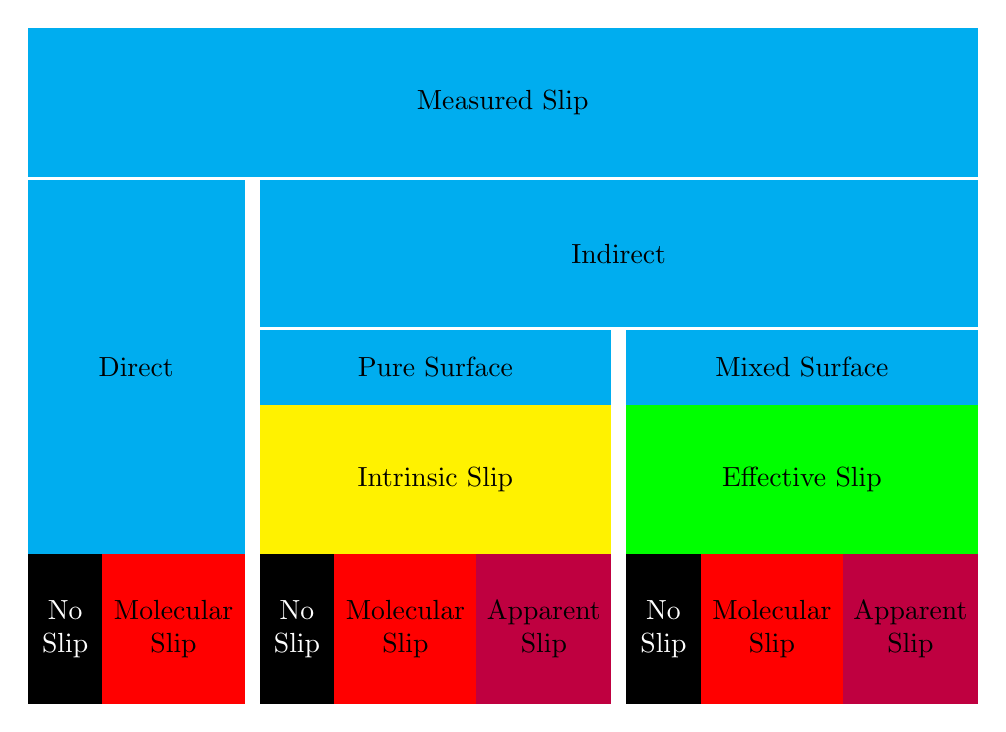
\begin{tikzpicture} [scale=0.95]
% Depending on some random factors, the rectangles may appear on screen to have faint white
% borders between them, or not.  The slight separation is good.  So I have made this explicit
% by lifting the bottom of Measured Slip and Indirect rectangles by 0.04 cm 

\fill[color=black] (0,0) rectangle node[color=white,align=center] {No\\ Slip} +(1,-2);
\fill[color=red] (1,0) rectangle node[color=black,align=center] {Molecular\\Slip} +(1.9,-2);

\fill[color=black] (3.1,0) rectangle node[color=white,align=center] {No\\ Slip} +(1,-2);
\fill[color=red] (4.1,0) rectangle node[color=black,align=center] {Molecular\\Slip} +(1.9,-2);
\fill[color=purple] (6,0) rectangle node[color=black,align=center]{Apparent\\Slip} +(1.8,-2);

\fill[color=black] (8,0) rectangle node[color=white,align=center] {No\\ Slip} +(1,-2);
\fill[color=red] (9,0) rectangle node[color=black,align=center] {Molecular\\Slip} +(1.9,-2);
\fill[color=purple] (10.9,0) rectangle node[color=black,align=center]{Apparent\\Slip} +(1.8,-2);

\fill[color=cyan] (0,0) rectangle node[color=black] {Direct} +(2.9,5);
\fill[color=cyan] (0,5.04) rectangle node[color=black] {Measured Slip} +(12.7,2);

\fill[color=yellow] (3.1,0) rectangle node[color=black] {Intrinsic Slip} +(4.7,2);
\fill[color=cyan] (3.1,2) rectangle node[color=black] {Pure Surface} +(4.7,1);

\fill[color=green] (8,0) rectangle node[color=black] {Effective Slip} +(4.7,2);
\fill[color=cyan] (8,2) rectangle node[color=black] {Mixed Surface} +(4.7,1);

\fill[color=cyan] (3.1,3.04) rectangle node[color=black] {Indirect} +(9.6,1.96);

\end{tikzpicture}
\end{center}

\vspace*{1em}
Note that the `Direct Measurement' category is there just for completeness --- experiments cannot presently verify molecular slip.


\section{Experimental Intrinsic Slip}

Probably the first credible experiments showing a slip effect are those by Erhard Schnell in 1956 \cite{Schnell1956}. In a series of careful experiments, Schnell treated glass capillaries with dimethyldichlorosilane to make them hydrophobic. The silicone layer decreased the capillary diameter by 0.01\% to 0.04\%. Nevertheless, at sub-turbulent velocities, the hydrophobic capillaries flowed 0\% - 5\% more water than otherwise-identical untreated capillaries. He attributed this excess flow to slip: '' ...this can only be explained by the slippage of water over the non-wettable surface."  Note that Schnell did not mention `slip length'.

After Schnell, various results of slip were reported. But, it is fair to say that it wasn't until the 21st century that truly believable evidence appeared.
Modern experimental techniques on slip progressed rapidly, starting from the 1990s, particularly the after widespread availability of the Atomic Force Microscope and its derivatives. The first of these new experiments exposed the usual host of subtle bugs and competing interpretations. See for example \cite{Pit2000}, \cite{CraigNetoWilliams2001}, \cite{BaudryCharlaix2001}, \cite{ZhuGranick2001}, \cite{Bonaccurso2002}, \cite{Neto2003}.

Hence, there is little point in trawling through the complete history. Instead, we focus on a `greatest hits' of slip measurement from recent years, by which time various experimental bugs had been ironed out.

The are three common experimental techniques used to study slip: Capillary flow, drainage force, and particle velocimetry.

\subsubsection*{Capillary Flow}

In this self-explanatory technique, the volumetric flow rates through capillaries are compared to standard theory.  The standard theory for flow in a straight circular pipe with no-slip boundary conditions is Poiseuille flow.  There is another analytic solution for the same pipe with Navier slip on the boundary. This solution is fitted to the experimental data; the parameter in question is the slip length.  Thus, an imputed slip length is found.

\subsubsection*{Drainage Force}

In this technique, a tiny sphere is repeatedly slammed onto the test surface. As the sphere nears the surface, the fluid is squeezed out of the way.  The force required to squeeze the fluid depends on the slipperiness of the test surface.  A theoretical model due to Vinogradova is used to predict the force, with slip length as the adjustable parameter; by fitting the model to the data, a slip length is inferred. In practice, the sphere is mounted on a cantilever, and driven in an oscillatory fashion, with force being calculated by the deflection of the cantilever.

An Atomic Force Microscope (AFM) in tapping mode is often used, as well as a similar purpose-built apparatus known as the Surface Force Apparatus (SFA).  This technique is very sensitive to inaccuracies in the position of the sphere relative to the surface.  Recent results use cunning techniques to determine this accurately.

\subsubsection*{Particle Velocimetry}

In this technique, thousands of tiny fluorescent particles are dumped in the flow.  Various clever techniques are used to track the particles, and infer their velocity.  The particles are small enough that Brownian motion is significant, so that it is necessary to average their velocity over a finite volume.  This obviously reduces the resolution of the inferred velocity field, so that this technique is still not `direct' enough to see molecular slip. Slip lengths are inferred by extrapolating a fitted velocity profile.

\subsection*{Recent Experimental Literature}

The no-slip boundary condition of classical fluid mechanics was based on observation. But given that slip effects were not noticed until the length scale of experiments became extremely small, are we sure that the no-slip condition \emph{really} holds?  So our first order of business is to verify the no-slip condition at the smallest possible scales.

\subsubsection*{No Slip}

Two recent papers show convincing evidence that the no-slip condition holds on hydrophilic surfaces.

The first, by Vinogradova and Yakubov in 2003 \cite{VinogradovaYakubov2003}, was a drainage force experiment, one of the first to use an AFM for extra sensitivity, rather than the usual SFA. A silicate glass sphere was tapped onto a hydrophilic silicon surface, both of which were molecularly smooth: rms roughness was 0.3 nanometers peak-to-peak. (For comparison, a water molecule is about the same size.) The experiment revealed no slip.

The trouble with this sort of experiment is the difficulty in determining the exact distance between sphere and surface.  This concern was taken very seriously in the second paper by Honig and Ducker, from 2007 \cite{HonigDucker2007}. They note: ``It is important to note that an error in determining the position of the solid-liquid interface ($h=0$) directly translates into an error in determining the slip length. In traditional colloidal probe measurements, the separation is not measured explicitly; the relative separation is determined from the sum of the displacement of a piezoelectric translation stage (``piezodisplacement") and the deflection of the cantilever. The zero of separation is inferred from the shape of deflection/piezodisplacement data." Problems include high force gradient near zero separation, thermal drift, and the fact that net separation is the small difference between two large measured displacements.

Honig and Ducker measure drainage forces with an AFM, but with what they claim is an explicit measurement of the separation between sphere and surface: ``We obtain the separation from the intensity of scattering of an evanescent wave by the particle." The particle --- the glass sphere of diameter ~10$\mu$m, was hydrophilic, with an rms roughness of 0.7 nm peak-to-peak, and a typical maximum peak-trough roughness of 4.5 nm. The glass plate was also hydrophilic, with an rms roughness of 0.25 nm, and a typical peak-trough roughness of 1.5 nm. A highly-wetting sucrose solution was used, with $\theta<5^{\circ}$.

In six experiments, no slip was found, even at shear rates of 250,000 sec$^{-1}$. 

\subsubsection*{Apparent or Molecular Slip}

The same level (or even greater) of care was taken in drainage force experiments performed by Cecile Cottin-Bizonne \emph{et al} in 2005 \cite{Cottin-Bizonne2005}. They used a SFA, but measured the distance between sphere and surface with a capacitive sensor, to a resolution of 1 Angstrom(!). The force on the plane was measured by the deflection of the cantilever on which it was mounted, with a resolution of 1 Angstrom.  The sphere was hydrophilic, while the plane was rendered hydrophobic by silanization with octadecyltrichlorosilane. The plane was examined with an AFM, revealing a peak-to-peak roughness of 1 nm.  Experiments were carried out in a clean and thermally isolated room.

With this setup, an implied slip of $19 \pm 2$ nm was measured. She emphasizes that the value ``does not depend on any pre-estimated values of liquid properties (viscosity, diffusivity of optical tracers) or of the geometry of solid surfaces, unlike data analysis used in AFM experiments or fluorescence measurements".  She further notes that early high-slip results were probably due to nanobubbles from cavitation or contamination with platinum nanoparticles. She finally notes that changing the environment to a clean room changed the results drastically(!).

\vspace{1em}
It is worth noting that `conventional' drainage force techniques continue to improve.  A very recent (2011) paper by Neto \emph{et al} \cite{ZhuAttardNeto2011} develops a `best practice experimental protocol' for studying slip with an AFM.  In a conventional AFM device, a piezoelectric element drives a small platform down towards the test surface.  To the platform are mounted a laser, a photodiode and a cantilever spring.  On the end of the cantilever is a small sphere --- a colloid; hence the apparatus is known as a colloidal probe.  When the colloid encounters hydrodynamic resistance, or hits the surface, the cantilever deflects.  This deflection is optically detected by the photodiode. Thus, the raw outputs of a typical AFM are the displacement of the piezo element and the photodiode voltage.

Obviously, the colloid-surface distance is not directly measured, it is inferred from raw data.  This paper identifies two problems. First, the platform flexes, causing the laser and photodiode to move relative to each other, causing a spurious deflection signal.  Second, when the colloid hits the surface, it scrapes sideways along the surface slightly.  The resulting friction causes a deflection of the cantilever in addition to the deflection caused by the normal force.  Neto \emph{et al} quantify and correct for these effects in their processing of the raw data.

With this protocol, they study slip in di-$n$-octylphthalate, and find a reproducible slip length in the range 24 - 31 nm.  The occasional slip length of  $\sim$ 60 nm prompts them to inspect the surface, \emph{after} the slip experiments.  They find contamination by nanoparticles about 20 nm in diameter, and note that this causes a false value for the zero of separation, which explains the occasional  anomalously high slip measurement.


\vspace{2em}
Turning now to particle velocimetry techniques, Huang \emph{et al} in 2006 \cite{Huang2006}  presented a fairly standard application of this method, but with some care taken to prevent the formation of nanobubbles: Purified water was used, which was degassed by exposure to a vacuum for 30 minutes.
200 nanometer diameter tracer particles were dispersed in the water, which flowed down channels etched in PDMS plastic.  Some channels were rendered hydrophobic by silanization with octadecyltrimethylsilane. The hydrophilic surfaces had rms roughness of 0.47 nanometers, while the hydrophobic surfaces has an rms roughness of 0.35 nanometers.

Total Internal Reflection Velocimetry was used to infer slip lengths for various shear rates. Hydrophilic surfaces showed slip lengths of 26 to 57 nm.  Hydrophobic surfaces showed slip lengths of 37 to 96 nm. If we assume the hydrophilic slip lengths are experimental artefact, then the true slip length is the extra slip length due to hydrophobicity.  Then, a true slip length of about 20 nm was obtained for shear rates in the range 300 - 1500 seconds$^{-1}$. At shear of 1800 sec$^{-1}$, the slip length rose to 54 nm. At low shear --- 200 sec$^{-1}$ --- the slip length was a mere 7 nm. With experimental uncertainty taken into account, an upper limit of 150 nm for a slip length is presented.

\vspace*{1em}
The problems of shear were eliminated in another particle velocimetry paper by Joly \emph{et al} also from 2006 \cite{Joly2006}.  In this work, water containing fluorescent particles of typical diameter 200 nm was confined between two surfaces, of roughness 1 nm peak-to-peak. There was no macroscale flow, only thermal diffusion.  The diffusion coefficient $D$ was calculated by measuring the residence time of the particles in a detection volume, using fluorescence correlation spectroscopy. If the surfaces are hydrophilic, the particle mobility should be strongly reduced by the proximity of the wall.  A finite element numerical solution to the Stokes equation gave a theoretical prediction for the mobility. For hydrophilic walls, theory and experiment agreed. For hydrophobic silanized walls, theory agreed with experiment if the prediction included a slip length of $18 \pm 5$ nanometers.

These results are shear-free, ruling out flow-induced nucleation of nanobubbles.

\vspace*{1em}
Another complication of shear flow is that it can increase the effective diffusivity of particles --- an effect known as Taylor dispersion. This complication is addressed in a 2009 paper by Vinogradova \cite{Vinogradova2009}. Glass capillaries, with rms roughness 0.3 nanometers, and silanized capillaries with rms roughness 0.7 nanometers were tested. Fluorescent nanoparticles were dumped in the flow, and their trajectories traced by double-focus fluorescence cross-correlation.  When the predicted Taylor dispersion velocity was subtracted from the observed particle velocity, no slip was observed for hydrophilic capillaries, and a slip length of no more than 80 - 100 nanometers for hydrophobic capillaries.

Vinogradova notes that while the apparent slip length depended on shear rate, the true slip length remained constant.  Finally, she notes that particle velocimetry is not expected to be capable of detecting slip lengths of a few tens of nanometers. 

\subsubsection*{Molecular Slip?}

A tantalizing glimpse of molecular slip is shown in a 2003 paper by Becker and Mugele \cite{BeckerMugele2003} --- but not with water.  Rather, they do drainage force experiments with octamethylcyclotetrasiloxane (OMCTS), a much larger molecule than water. The authors were primarily interested in the layering of fluid molecules in confined geometries.  Using a SFA to measure drainage force, they were able to observe discrete jumps in the force, as individual molecular layers escaped. They calculated that the momentum transfer (viscosity) between confined liquid layers was close to the bulk value, and that the solid/liquid equivalent viscosity was 18 times higher.  They did not mention `slip' or `slip length', but the solid/liquid `viscosity' can be interpreted as a friction coefficient $k$, with $b \propto k^{-1}$. Thus, if their interpretation of the experiments is correct, they have found molecular slip. 


\subsubsection*{Conclusions}

These modern, sophisticated experiments investigate slip on atomically flat --- rms roughness $< 1$ nanometer --- solid surfaces, with efforts made to reduce contamination by nanobubbles.  They show no slip on hydrophobic surfaces. For the hydrophobic case, an undeniable intrinsic slip length is present. Two different particle velocimetry studies put an upper limit on intrinsic slip length on the order of 100 nm.  Four different techniques produce results consistent with a slip length in the range $18 \pm 6$ nanometers, at least for moderate shear rates.

In general, no experiment provides direct evidence of molecular slip in water, but these experiments eliminate various confounding factors, leaving molecular slip as a distinct possibility.

\section{Theoretical Intrinsic Slip}

Theoretical arguments for slip are somewhat thin on the ground. Computer experiments, in the form of molecular dynamics (MD) simulations, form the backbone of theoretical work.

\subsection*{Molecular Dynamics}



Molecular Dynamics simulations involve the computer simulation of systems of particles governed by Newtonian mechanics.  Each particle has a position and momentum, and a net force on it due to the interaction with neighbouring particles. Time is sliced into discrete timesteps. At each timestep, the force on each particle is calculated, then the (instantaneous) acceleration, then the resulting translation. Then the position of each and every particle is updated simultaneously, using the calculated translations. The process is then repeated at the next timestep.

The technique is rightly called a computer \emph{experiment}, since the global behaviour is not predictable in advance.  Emergent phenomena such as melting, crystallization, annealing, etc. have been very successfully studied with MD.

Molecular Dynamics simulations differ in their choice of interaction. A very popular choice is the Lennard-Jones interaction, because it is computationally cheap and physically sound: the interaction features an equilibrium distance $\sigma$ between the the particles, a strong repulsion at shorter distances, and a weak attraction at longer distances.  This models dipole-dipole Van der Waals forces quite well.

\vspace*{1em}
Since the power of MD studies depends on Moore's Law, the first serious MD study of the fluid boundary condition appeared in 1990, a paper in Phys. Rev. A by Thompson and Robbins \cite{ThompsonRobbins1990}.
This featured a Lennard-Jones fluid under Couette shear, in conditions equivalent to a compressed fluid about 30\% above melting temperature. This was a qualitative study of the effects of varying two parameters: the wall-fluid interaction strength, \ewf, and the wall \emph{density.}

The wall is composed of stationary atoms. The separation between them can be arbitrarily set to any fraction or multiple of $\sigma$. The wall density is the inverse of separation distance. As the wall density tends to infinity, (separation diminishes to zero), the wall structure asymptotes to a \emph{flat plane.} In this case, the force between fluid atom and wall is always \emph{perpendicular} to the wall. Thus, the bounce of atoms off the wall will be \emph{specular reflection} --- no change in tangential momentum. This is the case of perfect slip; no transfer of tangential momentum. Thompson \& Robbins confirm that perfect slip obtains, regardless of the strength of \ewf.

\vspace*{1em}

\begin{center}
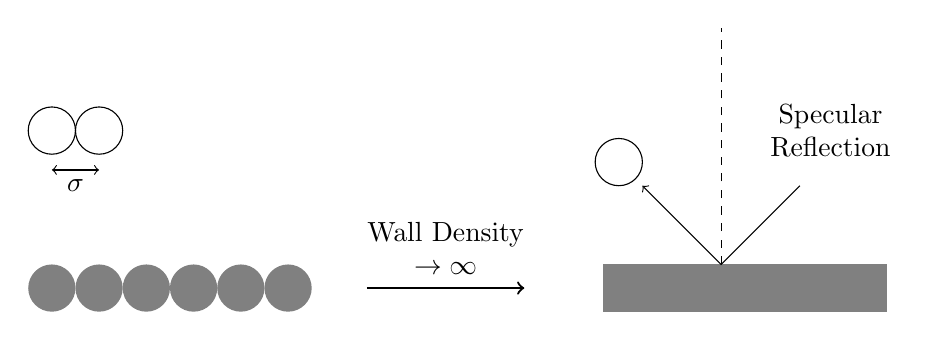
\begin{tikzpicture}

\foreach \x in {0,1,2,3,4,5}
     \fill[color=gray] (\x*0.6,0) circle (3 mm);

\draw (0,2) circle (3 mm);
\draw (0.6,2) circle (3 mm);
\draw[<->] (0,1.5) -- node[below]{$\sigma$} +(0.6,0);

\draw[->, thick] (4,0) -- (6,0);
\node at (5,0.5) [align=center] {Wall Density\\ $\rightarrow \infty$};

\fill[color=gray] (7,0.3) rectangle (10.6, -0.3);
\draw[dashed] (8.5,0.3) -- +(0,3);
\draw[->] (9.5,1.3) -- (8.5,0.3) -- (7.5,1.3);

\draw (7.2,1.6) circle (3 mm);

\node at (9,2) [align=center, right] {Specular\\ Reflection};
\end{tikzpicture}
\end{center}

\vspace*{1em}
As the wall density decreases, the wall gains some `texture', and fluid atoms can be given a sideways kick by the peaks of the wall.  Momentum transfer is now possible, and perfect slip no longer holds.
When the wall density is equal to fluid density, (wall atom separation is $\sigma$), Thompson \& Robbins observe the no-slip condition. At equal density, fluid atoms can attach epitaxially to the wall.  If \ewf is strong enough, one or two layers of fluid atoms lock to the wall.
\vspace*{1em}

\begin{center}
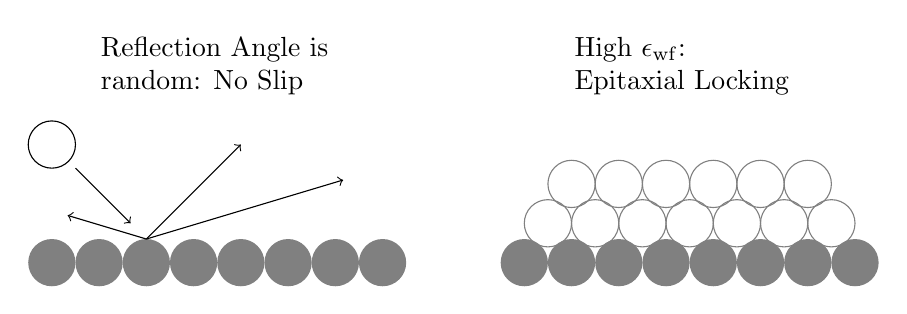
\begin{tikzpicture}

\foreach \x in {0,1,2,3,4,5,6,7, 10,11,12,13,14,15,16,17}
     \fill[color=gray] (\x*0.6,0) circle (3 mm);

\foreach \x in {10,11,12,13,14,15,16}
     \draw[color=gray] (\x*0.6 + 0.3,0.5) circle (3 mm);
 
\foreach \x in {10,11,12,13,14,15}
     \draw[color=gray] (\x*0.6 + 0.6,1) circle (3 mm);
     
\node at (8,2.5)[align=left] {High $\epsilon_{\mathrm{wf}}$:\\ Epitaxial Locking};
         
\node at (0.5,2.5)[right,align=left] {Reflection Angle is\\ random: No Slip};

\draw     (0,1.5) circle (3 mm);
\draw[<-] (1.0,0.5) -- +(-0.7,0.7);
\draw[->] (1.2,0.3) -- +(1.2,1.2);
\draw[->] (1.2,0.3) -- +(2.5,0.75);
\draw[->] (1.2,0.3) -- +(-1,0.3);

\end{tikzpicture}
\end{center}

\vspace*{1em}

At a wall density of 2.52 times the fluid density (solid atom separation is 0.397 $\sigma$), Thompson \& Robbins found that fluid layering was reduced, and slip increased. At higher \ewf, however, the fluid atoms again formed a close-packed layer, but with a periodic structure that was a harmonic of the wall structure. At the highest \ewf, the fluid atoms locked epitaxially to the wall, in a state of elastic strain.

\vspace*{1em}

\begin{center}
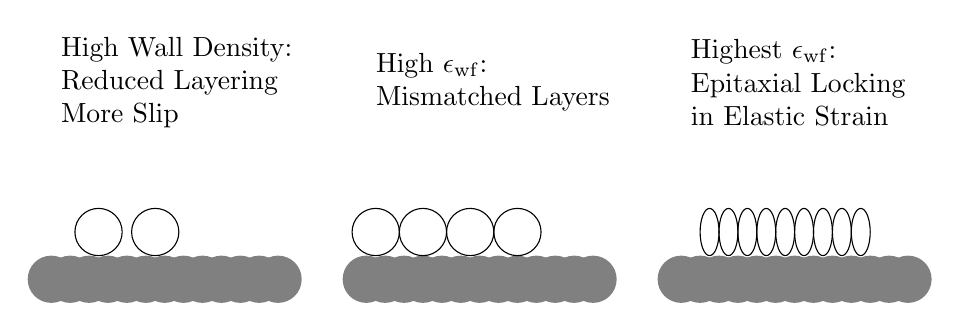
\begin{tikzpicture}

\foreach \d in {0,4,8}
    \foreach \x in {0,1,2,3,4,5,6,7,8,9,10,11,12}
        \fill[color=gray] (\x*0.24 + \d,0) circle (3 mm);

\foreach \d in {2,5}
    \draw (0.12 + 0.24*\d, 0.6) circle (3 mm);

\node at (0,2.5)[right,align=left] {High Wall Density:\\Reduced Layering\\More Slip};

\foreach \x in {0,1,2,3}
    \draw (4.12 + 0.6*\x, 0.6) circle (3 mm);

\node at (4,2.5)[right,align=left] {High $\epsilon_{\mathrm{wf}}$:\\Mismatched Layers};

\foreach \x in {1,2,3,4,5,6,7,8,9}
    \draw (8.12 + 0.24*\x, 0.6) ellipse (1.2mm and 3mm);

\node at (8,2.5)[right,align=left] {Highest $\epsilon_{\mathrm{wf}}$:\\
Epitaxial Locking\\ in Elastic Strain};

\end{tikzpicture}
\end{center}

\vspace*{2em}

Following this qualitative work, Thompson and Troian report some quantitative results from very similar Lennard-Jones simulations in a 1997 Nature article \cite{ThompsonTroian1997}. Again they vary the wall density $\rho_{\mathrm{wf}}$ and \ewf, (as a fraction of $\epsilon$, the fluid-fluid interaction strength) as well as $\sigma_{\mathrm{wf}}$, the equilibrium distance of wall and fluid atoms. Slip lengths in units of $\sigma$ are calculated for various regimes:

\vspace*{1em}
\begin{center}
\begin{tabular}{l l l l}
\ewf & $\sigma_{\mathrm{wf}}$ & $\rho_{\mathrm{wf}}$ & $b$ \\
0.6  & 1.0                    & 1                    & 0 \\
0.1  & 1.0                    & 1                    & 2 \\
0.6  & 0.75                   & 4                    & 4 \\
0.4  & 0.75                   & 4                    & 8 \\
0.2  & 0.75                   & 4                    & 18 \\
\end{tabular}
\end{center}
\vspace*{1em}

Now, $\ewf < \epsilon$ means that a fluid atom is more attracted to other fluid atoms than to the wall.  This could be interpreted as hydrophobicity. Hence, the data show that if epitaxial locking is easy, then slip is suppressed, even for a mildly hydrophobic surface. Likewise, the data show that if the density of stable attachment sites is too high for epitaxial locking, then slip results.

But the real story is the shear dependence of slip. The fluid is in a Couette flow regime, with top and bottom surfaces moving with equal and opposite velocities.  At low shear rates, the slip length is a constant plateau, but at some critical shear rate, the slip length diverges, i.e. goes berserk heading for infinity. The critical shear rate depends on the regime.  Interestingly, if the shear rates are normalised to their critical shear rate, and the slip lengths normalised to their plateau value, then the slip length versus shear rate data for all regimes lie \emph{on a single curve.}

Thompson \& Troian attempt to explain this ``remarkable collapse of the data" with a single parameter $R$ describing the roughness of the potential surface. A test particle at a fixed height experiences a potential $\phi(x,y)$. Define $A$ as the area integral of $\phi(x,y)$, and $A_{\infty}$ as the area integral of the limiting case of a flat plane (infinite atom density). Then

\begin{equation}
R = \frac{A}{A_{\infty}} - 1
\end{equation}

With a wall moving at velocity $v$, a test particle experiences perfect slip for $v>v_{c}$, some critical velocity. They find that $v_{c}$ scales as $R^{1/2}$ for a wide range of parameters. In the real fluid (with hundreds of particles) they find $v_{c}$ scales as a power of $R$ with an exponent close to $3/4$.

Thompson \& Troian think it is reasonable to assume that $v_{c}$ is set by the liquid-solid interaction timescale, so that increasing density should lead to larger $v_{c}$.  They are surprised to find the reverse.

But this is an odd expectation. Assuming that the average approach velocity of impacting particles remains the same, a faster moving or more dense surface increases the probability of a particle interacting with a peak, thus experiencing a closer-to-normal force, causing closer-to-specular reflection -- i.e. perfect slip.  In the same way, an electric fan seems `solid' to the inquisitive fingers of a child.

\vspace*{1em}

Barrat and Bocquet \cite{BarratBocquet1999} study flow in both Poiseuille and  Couette regimes, using a Lennard-Jones fluid with an additional $c_{ij}$ parameter:

\begin{equation}
v_{ij} = 4 \epsilon \left[ \left( \frac{\sigma}{r}\right)^{12}
 - c_{ij} \left( \frac{\sigma}{r} \right)^{6} \right]
\end{equation}


They use $c_{FF} = 1.2$ for fluid-fluid interactions, making the fluid more cohesive than the usual Lennard-Jones fluid. They tweak the wetting properties via the $c_{FS}$ fluid-solid parameter.  There are several ways to calculate the contact angle from this parameter.  The most accurate way gives $c_{FS}=0.5 \rightarrow \theta= 140^{\circ}$ and $c_{FS} = 1.0 \rightarrow \theta = 90^{\circ}$.

A hydrophobic liquid ($\theta = 140^{\circ}$) requires a pressure $P_{0}$ to jam it down the pipe (to overcome Laplace pressure). At high pressure, $P/P_{0}=16.4$, the fluid exhibited the same higher-density layering at the wall as seen in hydrophilic liquids.  At a lower pressure, $P/P_{0}$, the fluid showed a \textbf{strong density depletion} near the wall.  The slip length varied tremendously over this pressure range: from $b = 8\sigma$ for $P/P_{0} = 16.4$ to over $40\sigma$ for $P/P_{0} \sim 0$.

Less hydrophobic fluids showed less slip, and less pressure dependence. A $c_{FS}>0.7$ ($\theta \leq 120^{\circ}$) gave slip lengths of a couple of $\sigma$ only.

Note that the position of the hydrodynamic boundary was treated as an adjustable parameter.  It turned out to be located one atom width into the liquid.  The arbitrary nature of the boundary position was not fully appreciated by the experimental community until almost 10 years after this sort of theoretical paper.

\subsubsection*{Correlation Function Tuned by Molecular Dynamics}

In this sophisticated theoretical paper \cite{BocquetBarrat1994}, Bocquet and Barrat start by constructing a phenomenological model of a fluid: Each infinitesimal volume of fluid has a \emph{momentum.} This momentum field is subject to fluctuations, which quickly dissipate, obeying the diffusion equation. Further, any pressure gradient is proportional to the gradient of momentum divergence. Adding relevant physical constants, and dividing through by the volume element to get a momentum \emph{density,} $\vec{j}(\vec{r},t)$, in the bulk:
\begin{equation}
 \partial_{t} \vec{j}+\nabla P - \frac{\xi+\eta/3}{\rho_{0}}\nabla
 [\nabla \cdot \vec{j}] - \frac{\eta}{\rho_{0}} \nabla^{2} \vec{j} = 0
\end{equation}
And on the boundary, Navier slip holds:
\begin{equation}
\vec{j}_{\parallel} = b_{\mathrm{wall}} \frac{\partial}{\partial \vec{n}}
 \vec{j}_{\parallel} , \;\;\;\;\; \vec{j}_{\perp} = 0
\end{equation}
Bocquet \& Barrat now consider a fluid contained between two $x,y$ planes separated by distance $h$. Slip lengths $b_{0}$ and $b_{h}$ hold on the lower and upper planes, respectively.

A great simplification is to introduce the `transverse momentum density':

\begin{equation}
j_{x}(z,t) = \frac{1}{L_{x}L_{y}} \int \int dx dy \; j_{x}(\vec{r},t)
\end{equation}
And similarly for $j_{y}(z,t)$.

With the pressure gradient essentially integrated out, this field obeys the diffusion equation + Navier slip conditions:
\begin{gather}
\left[ \partial_{t} - \frac{\eta}{\rho_{0}} \partial_{z}^{2} \right]
j_{x}(z,t) = 0
\\
j_{x}(z,t)|_{z=z_{0}} = b_{0} \partial_{z} j_{x}(z,t)|_{z=z_{0}} , \;\;\;\
\;\;  j_{x}(z,t)|_{z=z_{0}+h} = -b_{h} \partial_{z} j_{x}(z,t)|_{z=z_{0}+h}
\end{gather}

The cunning trick is to work with the time-dependent correlation function:

\begin{equation}
C(z,z',t) = \left< j_{x}(z,t), j_{x}(z',0) \right>
\end{equation}
where angle brackets denote a thermodynamic average.

Finally, this equilibrium correlation function also obeys the diffusion and Navier slip equations:

\begin{gather}
\left[ \partial_{t} - \frac{\eta}{\rho_{0}} \partial_{z}^{2} \right]
C(z,z',t) = 0 \quad :\;\; 0<z<z_{0}+h 
\\
C(z,z',t)|_{z=z_{0}} = b_{0} \partial_{z} C(z,z',t)|_{z=z_{0}}
\\
C(z,z',t)|_{z=z_{0}+h} = -b_{h} \partial_{z} C(z,z',t)|_{z=z_{0}+h}
\end{gather}
There is a general solution (details omitted):

\begin{equation}
C(z,z',t) = f(b_{0}, b_{h}, h)
\end{equation}

That is, the correlation function is a (hideous) function of \emph{slip length} and \emph{channel width.} The parameter `channel width' is equivalent to `effective position of the boundary condition'.  Bocquet \& Barrat note that in Couette flow, the two parameters are not independent, but in general may be.

Now, one can directly observe a molecular dynamics simulation, and calculate the correlation function of the simulation. Bocquet \& Barrat carry out an equilibrium MD simulation --- no shear or pressure, just thermal motion --- and harvest the correlation function.  The parameters of the theoretical correlation function are tweaked until it best fits the MD correlation function.

Thus, a slip length and effective boundary position are derived from MD, without inducing and measuring velocities, therefore eliminating  shear dependence from the slip effect.

The first MD experiment used a repulsive-only fluid/wall interaction -- a `soft sphere' model. The wall had a corrugation with wavelength of $1 \sigma$, and a varying amplitude:

\vspace*{1em}
\begin{center}
\begin{tabular}{lll}
Amplitude      & Slip Length      & BC Position \\
0  (flat)      & $\infty$         & 1.60 \\
0.01           & $40 \pm 2.5$     & 1.60 \\
0.02           & $7.20 \pm 0.05$  & 1.60 \\
$>0.03$        & $0.00 \pm 0.02$  & 1.60 \\
\end{tabular}
\end{center}

\vspace*{1em}
The remarkable result is that even a tiny corrugation --- depth 0.03 $\sigma$ --- is enough to completely suppress slip. Also, the hydrodynamic BC is located about one atom width inside the fluid.

A second Lennard-Jones MD simulation with a corrugation depth of 0.2 $\sigma$ was done.  Particles locked epitaxially to the solid, with zero slip, and a BC located two atom widths inside the fluid.

As a final test, Bocquet \& Barrat do a conventional Couette flow MD simulation, extracting velocity profiles to infer slip lengths. The results agreed with the equilibrium method.

\subsubsection*{Depletion Layer and Drainage Force}
In a landmark paper from 1995 \cite{Vinogradova1995}, Olga Vinogradova studied the `drainage of a thin liquid film confined between hydrophobic surfaces'. The results are in two main parts.

\paper{The Boundary Conditions on the Hydrophobic Surface:}
Vinogradova looks at the two candidates for intrinsic slip: molecular slip and apparent slip.
She notes that molecular slip was first proposed by Tolstoi back in 1952; his theories were revisited by Blake in 1990, who predicted the slip effect on flow rate in a capillary.  These predictions sometimes matched experiment, but Ruckenstein and Rajora in 1993 noted that the implied surface diffusion coefficients are several orders of magnitude larger than those observed even for gases.

Having found evidence for molecular slip wanting, she considers apparent slip.  A `gas gap' has been suggested as the cause, but this is not experimentally confirmed. Another model of apparent slip is the decrease in viscosity in a boundary layer close to the hydrophobic surface. Crucially, she states: ``this fact follows from numerical simulation data, as well as from the direct experimental results obtained by the blowoff method. (Derjaguin \emph{et al} 1993)". From this firm foundation, Vinogradova notes that if the boundary layer of thickness $\delta$ has an average viscosity $\mu_{\mathrm{slip}}$, smaller than the bulk viscosity $\mu_{\mathrm{bulk}}$, then an order of magnitude estimate of apparent slip length is:

\begin{equation}
b= \delta \left( \frac{\mu_{\mathrm{bulk}}}{\mu_{\mathrm{slip}}} - 1 \right)
\end{equation}
This is of course would be well defined only if $\delta$ and $\mu_{\mathrm{slip}}$ were known.

This model covers the case of bubbles on the surface, and Vinogradova observes that much experimental slip may be due to dissolved gas, causing bubbles to form on the surface or in microcavities.

\paper{Solution of the Drainage Problem:}
Vinogradova considers two perfectly spherical (no roughness) solids being squeezed together at (instantaneous) velocity $v$ in a Newtonian fluid of viscosity $\mu$. The two spheres have radii $R_{1}$ and $R_{2}$, and slip lengths $b$ and $b(1+k)$ on their surfaces, respectively. After a lovely piece of classical mathematical physics, she derives a formula for the drainage force
$F_{z}$ in terms of separation $h$:

\begin{equation}
F_{z} = - \frac{6 \pi R_{e}^{2} \mu v}{h} f^{*}
 \;\;\;\; \mathrm{where}\;\;\;R_{e} = \frac{R_{1}R_{2}}{R{1}+R_{2}} = 
 \frac{R_{1}}{\frac{R_{1}}{R_{2}} + 1}
\end{equation} 

 In the limiting case of a hydrophobic sphere interacting with a similar one:
 
\begin{equation}
f^{*} = (2)\frac{h}{6b} \left[ \left(1 + \frac{h}{6b} \right)
 \ln \left(1 + \frac{6b}{h} \right) - 1 \right]
\end{equation}
Note that $R_{e} = R_{1}$ in the case of a sphere approaching a flat plane ($R_{2}=\infty$).

This formula is used by the experimental community in all subsequent drainage force experiments.

\subsubsection*{Depletion Layer as a Gas Layer}

In a wonderfully readable little paper from 2002 in Langmuir \cite{deGennes2002}, de Gennes derives the slip length expected of a hypothetical gas layer.  De Gennes finds the then-recent very high experimental slip lengths ``unexpected and stimulating."  (These experiments are now suspected of being contaminated with bubbles; de Gennes is thus prescient in his gas layer theory.) ``This led us to think about unusual processes which could take place near a wall.  In this Letter, we discuss one (remote) possibility: the formation of a gaseous film at the solid/liquid interface.

``The source of the film is unclear: when the contact angle is large ($\theta \rightarrow 180^{\circ}$), a type of flat bubble can form at the surface with a relatively low energy.  But this energy is still high compared to the thermal energy $k_{B} T$."

With these caveats stated, de Gennes derives the slip length expected for a bulk fluid of viscosity $\eta$, sliding over a gas layer of density $\rho$, and uniform thickness $h$. Layer thickness $h$ is assumed to be greater than the molecule size, but smaller than the mean free path in the gas.

Unfortunately, there are a few issues: there seem to be several typographical errors, and the result is stated in terms of the somewhat unfamiliar $\bar{v}_{z}$, which is apparently defined as the mean \textbf{absolute value} of the normal component of gas particle velocity (the simple mean is zero).  To resolve the inconsistencies, and restate the result in a more standard way, in Appendix A we derive the result from scratch, in terms of the mean \emph{speed} in the gas, $\bar{v}$.  We find:
\begin{equation}
b = \frac{4 \eta}{\rho \bar{v}}
\end{equation}
(We show that this is equivalent to the result of de Gennes.)

Note that $b = 4 \eta/ \rho \bar{v}$ is the slip length parameter found in the boundary condition located at the \textbf{bottom of the fluid.}  If $b$ is instead regarded as a property of the \emph{solid} surface, then the gas layer thickness $h$ must be subtracted.  We shall see that this is negligible:

Plugging in typical values: $\rho$ = 1 kg/m$^{3}$, $\bar{v}$ = 476 m/s, $\eta$ = $10^{-3}$ kg/ms, we get $b$ = 8 $\mu$m. De Gennes: ``Thus, a gas film can indeed give a very large slip length.  Our calculation assumed complete thermalization at each particle/boundary collision.  If we had some nonzero reflectance (especially on the solid surface), this would increase $b$ even more."

De Gennes notes that the amount of gas required is very small, but that a ``process which could generate such films remains obscure."  Serendipitously, the very next year, Andrienko \emph{et al} proposed an abstract description of just such a process.


\subsubsection*{Phase Separation causing a Depletion Layer}

The depletion layer theory of slip was given another boost by some fairly abstract theorising by Andrienko \emph{et al} in a 2003 paper \cite{Andrienko2003}.  Rather than focusing on what the low-viscosity boundary \emph{is,} they take an agnostic, abstract approach: They considered a toy model of a generic admixture of two different fluids, whose viscosities differ by the (arbitrary) ratio 1:3.  A `phase field' approach was used, in which an order parameter $\phi$ varies over space.  Here, $\phi$ was the fraction of low-viscosity fluid in an infinitesimal volume.

The unmixing of the fluid is driven by energy (as always).  Andrienko \emph{et al} start with a free energy functional --- the semigrand potential. With this functional set up, they consider the physical case of Couette flow between two fairly close plates. Variation of the functional yields an Euler-Lagrange equation and a boundary condition:

\begin{gather}
 k^{2} \frac{\partial^{2}\phi}{\partial z^{2}} + 
\frac{1}{2}T\ln \frac{1+\phi}{1-\phi} + \mu = 0
%\end{equation}
\\
%\begin{equation}
\pm k \frac{\partial \phi}{\partial z} + h + \gamma \phi|_{z= \pm L/2} = 0
\end{gather}
Where $k$ is inexplicably undefined, $T$ is temperature, $\mu$ is chemical potential, $h$ measures attractiveness of the surface to the low-viscosity fluid, and surface coupling $\gamma$ captures the fact that a molecule on the surface has fewer neighbours than a molecule in the bulk.

These equations were solved numerically with Fortran using the relaxation method. With the $\phi$ field solution, the viscosity field was obtained by simply assuming that viscosity is a linear combination of the pure viscosities. Finally the Couette flow field was solved for the viscosity field.

The big result is that above a certain temperature, a layer of the low-viscosity fluid suddenly forms on the surface.  Andrienko \emph{et al} call this a `prewetting transition'.  This causes the sudden emergence of a significant slip length.  As temperature increases above this critical temperature, more mixing occurs, reducing the viscosity contrast, thus reducing slip length.

Andrienko \emph{et al} believe this mean-field toy model to be valid for liquid-gas systems, binary mixtures, and polymer mixtures in the long wavelength approximation.  Thus, large slip is predicted for those systems.

\subsection*{Conclusions}

Intrinsic slip certainly exists, on atomically-flat clean surfaces.  Molecular dynamics simulations show a variety of interesting phenomena, including molecular slip, and a depletion layer causing apparent slip.  The depletion layer model is an excellent candidate for a physical explanation.  Intrinsic slip lengths of roughly 20 nanometers are credibly measured. 

In the next chapter, we turn to flow over mixed-slip surfaces, 
where the intrinsic slip length is different on different parts of the surface.   


\bibliography{Lund_Thesis.bib}
\bibliographystyle{plain}

\end{document}
